%% LLT: Turn off some annoying warnings...
\RequirePackage{silence}
\WarningFilter{titlesec}{Non standard sectioning command}
\WarningFilter{scrreprt}{Usage of package}
\WarningFilter{scrreprt}{Activating an ugly workaround}

% *********************************************************
% CHOOSE THEME (ucph, sund, science, hum, samf, jura, teo)
% *********************************************************

% NOTE: can ONLY RUN UCPH theme with the 2018(legacy) version. Can be changed under Menu

\newcommand{\thesisTheme}{ucph} % to colortheme and titlepage image


% *********************************************************
% DOCUMENT CLASS
% *********************************************************
\documentclass[%
	paper=A4,					% paper size
	12pt,						% font size
	twoside=true,				% two-sided printing
	openright,					% doublepage cleaning ends up right side
	parskip=full,				% spacing value / method for paragraphs
	chapterprefix=true,			% prefix for chapter marks
	headings=normal,			% size of headings
	bibliography=totoc,			% include bib in toc
	listof=totoc,				% include listof entries in toc
	titlepage=on,				% own page for each title page
	captions=tableabove,		% display table captions above the float env
	draft=false,				% value for draft version
	abstract=on,                % abstract title on/off
]{scrreprt}
\usepackage[utf8]{inputenc}
\usepackage[english]{babel}     % adjust the language

% **************************************************
% COMMANDS FOR REUSE
% **************************************************

% Thesis
\newcommand{\thesisTitle}{PhD title}
%\newcommand{\thesisSubtitle}{A case study for all faculties at University of Copenhagen}
\newcommand{\thesisName}{Author Name}
\newcommand{\thesisSubject}{PhD Thesis}
\newcommand{\thesisDate}{Month Year}
\newcommand{\thesisVersion}{1. Version © Author Name, Month Year}

\newcommand{\thesisGradSchool}{This thesis has been submitted to the Graduate School at Faculty of Health and Medical Sciences, University of Copenhagen}

% Supervisors & Collaborators
\newcommand{\thesisSupervisor}{Supervisor 1\\Supervisor 2\\Superviros 3\\  [0.2 cm] 
%\textit{All:}\\ 
%\thesisFaculty 
%\\
%\thesisUniversity
}
\newcommand{\thesisAssessment}{Opponent 1 (Chairperson)\\University, Country  \\ [0.3 cm] Opponent 2\\ University, Country \\[0.3 cm] Opponent 3\\ University, Country}
\newcommand{\thesisCollab}{If any?}

% University of Copenhagen
\newcommand{\thesisUniversity}{\protect{University of Copenhagen}}
\newcommand{\thesisFaculty}{Faculty of Health and Medical Sciences}
\newcommand{\thesisDepartment}{Department of Veterinary and Animal Sciences}
\newcommand{\thesisSection}{Section of Animal Welfare and Disease Control}
\newcommand{\thesisCity}{Frederiksberg}
\newcommand{\thesisAddress}{Grønnegårdsvej 8}
\newcommand{\thesisPostal}{1870}
\newcommand{\thesisCountry}{Denmark}

% External institution: University of Sussex
\newcommand{\thesisUniSus}{\protect{University of xxx}}
\newcommand{\thesisUniSusDep}{Department of xx}


% *********************************************************
% PACKAGES
% *********************************************************

\usepackage[					% UCPH thesis style
    figuresep=colon,        
    sansserif=false,        
    hangfigurecaption=false,
    hangsection=true,       
    hangsubsection=true,    
    colorize=full,          
    colortheme={\thesisTheme},  % ucph, sund, science, hum, etc.?
    bibsys=biber,
    bibfile=references,       % defines your .bib file
    bibstyle=authoryear,        % refer to https://bit.ly/2YsvIJz
]{ucphthesis}
\hypersetup{					% setup the hyperref-package options
	pdftitle={\thesisTitle},	% 	- title (PDF meta)
	pdfsubject={\thesisSubject},% 	- subject (PDF meta)
	pdfauthor={\thesisName},	% 	- author (PDF meta)
	plainpages=false,			% 	-
	colorlinks=false,			% 	- colorize links
	pdfborder={0 0 0},			% 	-
	breaklinks=true,			% 	- allow line break inside links
	bookmarksnumbered=true,		%
	bookmarksopen=true			%
    }

% *********************************************************
% Cover page content
% *********************************************************
\subject{\vspace{4.5cm} \thesisSubject}
\title{\thesisTitle}
%\subtitle{\thesisSubtitle}
\author{\thesisName}
\date{\thesisDate \\ \vspace{3cm} { \small This thesis has been submitted to the Graduate School at Faculty of Health and Medical Sciences, University of Copenhagen. Date.\\}}



% ********************************************************* 
% THESIS CONTENT
% *********************************************************
\begin{document}

% -------------------------- 
% Front matter
% --------------------------
\pagenumbering{roman}
\pagestyle{empty}				            % no header or footers
\AddToShipoutPicture*{\TitleBackground}     % adding background picture
\maketitle                                  % making the title
% Cover back page
\AddToShipoutPicture*{\TitleWatermark} % adding watermark
%\hfill
{
	\small
	%\textit{\thesisTitle} \\
	%\thesisName \\
	%\thesisSubject, \thesisDate \\[1.5em]
	\textbf{Supervisors} \\
	\thesisSupervisor \\[1.5em]
	\textbf{Assessment Committee}\\
	\thesisAssessment \\[1.5em]
    \vfill
	\textbf{\thesisUniversity} \\
	\textit{\thesisFaculty} \\
	\thesisDepartment \\
	\thesisSection \\
	\thesisAddress,  \thesisPostal\ \thesisCity \\
	\thesisCountry \\[1.5em]
    %\thesisGradSchool \\[1.5em]
    \thesisVersion % add some copyright
}

\clearpage

\pagestyle{plain}

% Table of Contents (could also be just before Main Matter)
\setcounter{tocdepth}{2}		% define depth of toc
\tableofcontents				% display table of contents
    \clearpage

%\input{frontbackmatter/quotes.tex}          % INCLUDE Quotes. Quote has been included in preface
\pdfbookmark[0]{Preface}{Preface}
\chapter*{Preface and Acknowledgements}
\label{chap:preface}
\addcontentsline{toc}{chapter}{Preface and Acknowledgements}
%\vspace*{5cm}
%\Blindtext[1]

My preface and acknowledgements

\newpage
% Quote added here instead of seperate page. maybe a picture instead of the quote?
\textit{"Maybe I even want to quote someone?.."} \\
\newline
\rightline{Author} \\
\vspace{1cm}         % INCLUDE Preface
\pdfbookmark[0]{Summary}{Summary}
\chapter*{Summary}
\label{chap:summary}
\addcontentsline{toc}{chapter}{Summary}

This is my summary         % INCLUDE Abstract
\pdfbookmark[0]{Sammendrag}{Sammendrag}
\chapter*{Sammendrag}
\label{chap:sammendrag}
\addcontentsline{toc}{chapter}{Sammendrag}
Summary oversat      % INCLUDE Danish abstract
\pdfbookmark[0]{List of Figures}{List of Figures}
%\chapter*{List of Figures}
%\newpage % replace \cleardoublepage to ensure starting on odd pages
\cleardoublepage
\addcontentsline{toc}{chapter}{List of Figures}
\label{chap:list_figures}

\listoffigures   % INCLUDE List of figures
\pdfbookmark[0]{Tables}{Tables}
%\chapter*{List of Tables}
%\newpage % replace \cleardoublepage to ensure starting on odd pages
\cleardoublepage
\addcontentsline{toc}{chapter}{List of Tables}
\label{chap:list_tables}

\listoftables   % INCLUDE List of tables
\pdfbookmark[0]{Abbreviations}{Abbreviations}
\chapter*{Abbreviations}
\label{chap:abbreviations}
\addcontentsline{toc}{chapter}{Abbreviations}

% abbreviations can also be made directly wit a latex command

\begin{center}
\addtolength{\tabcolsep}{10pt} 
\begin{tabular}{ l l }
 AWD & Animal Welfare and Disease Control \\
 IVH & Institute of Veterinary Health
\end{tabular}
\addtolength{\tabcolsep}{-10pt}
\end{center}

%\newpage
\cleardoublepage % change to \newpage if Abbreviations cover 2 pages   % INCLUDE abbreviations
    \clearpage


% -------------------------- 
% Main matter
% --------------------------
\pagenumbering{arabic}			% arabic page numbering
\setcounter{page}{1}			% set page counter
\pagestyle{maincontentstyle} 	% fancy header and footer

\chapter{Background}
\label{chap:background}

This is my background.

EU made an animal health law in 2016 \autocite{EU2016}.


       % INCLUDE background
\chapter{Purpose and Outline}
\label{chap:purpose}

The purpose of this PhD study was to ...

          % INCLUDE purpose and aim
\chapter{General Introduction}
\label{chap:intro}


\section{Diseases}
My PhD thesis is about diseases


%%%%%%%%%%%%%%%%%%%%%%%%%%%%%%%%%%%%%%%%%%%%%%%%%%%%%%

\subsection{This specific disease}
This is a subsection about a specific disease


\begin{figure}[htp]
    \centering
    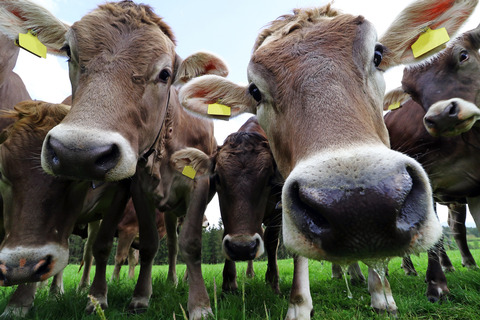
\includegraphics[width=12cm]{figures/cows_closeup.jpg}
    \caption{A cow from colourbox}
    \label{fig:cow}
\end{figure}




     % INCLUDE Introduction
\chapter{Summary of Materials and Methods}
\label{chap:materialsandmethods}

My materials and methods

\section{Data}
Add stuff


\subsection{Databases}
Add more stuff




 % INCLUDE M&M
\chapter{Summary of Results and Discussions}
\label{chap:results}

This is my results and discussions   % INCLUDE General Discussion
\chapter{Conclusion and Perspectives}
\label{chap:con}

This is my conclusions and perspectives       % INCLUDE Conclusion and perspectives
\chapter{Publications}
\label{chap:research_output}

Maybe you want a list with all of your publications?

\begin{itemize}
  \item \textbf{Me}, info about publication..

  \item \textbf{Also Me}, info about publication..

\end{itemize}

    % INCLUDE research output



% -------------------------- 
% Back matter
% --------------------------
\chapter{Bibliography}
\vspace{1cm}
\printbibliography[heading=none]

% This is based on the references.bib file.
% for own references, create a bib file and upload it
\chapter{Appendix A - Scripts}
\label{chap:scripts}

Maybe you want a chapter with your codings?

\chapter{Appendix B - MyData}
\label{chap:data}

Maybe I want to describe my data
\chapter{Appendix C - Publications and Manuscripts}
\label{chap:publications}

Manuscripts can be included by importing a pdf

\section{Manuscript I}


\section{Manuscript II}


\section{Manuscript III}
    % INCLUDE all prints

% ********************************************************* 
% END OF THESIS
% *********************************************************
\end{document}